\begin{questions}
\question{
$\exp(i\vec{G}\cdot \vec{T})  =1$
}
\begin{solution}
  Let's begin with the definition of the reciprocal basis vectors $b_i$
  \begin{equation}
    \bm{b}_i = 2\pi \frac{\bm{a}_j \times \bm{a}_k}{\bm{a}_i\cdot(\bm{a}_j \times \bm{a}_k)}\epsilon_{ijk},
    \label{b:rec}
  \end{equation}
  where $\epsilon_{ijk}$ is the Levy-Civitta symbol, and $\bm{a}_i$ are the direct basis vectors.
  Let's move forward and define this two vectors,
  \begin{equation}
    \bm{T} = n_1\bm{a}_1 + n_2\bm{a}_2 + n_3\bm{a}_3 \qquad n_i\in\mathbb{Z},
    \label{T}
  \end{equation}
  \begin{equation}
    \bm{G} = m_1\bm{b}_1 + m_2\bm{b}_2 + m_3\bm{b}_3 \qquad m_i\in\mathbb{Z}.
    \label{G}
  \end{equation}
  From eq. \ref{b:rec} it is easy to notice that $\bm{a}_i\cdot \bm{b}_j = 2\pi \delta_{ij}$, we will use this fact on the next step. Now, let's compute the following dot product
  \begin{equation}
    \begin{aligned}[b]
      \bm{G}\cdot\bm{T} &= (n_1\bm{a}_1 + n_2\bm{a}_2 + n_3\bm{a}_3)\cdot(m_1\bm{b}_1 + m_2\bm{b}_2 + m_3\bm{b}_3),\\
      &= n_1\bm{a}_1\cdot(m_1\bm{b}_1 + \cancelto{0}{m_2\bm{b}_2} + \cancelto{0}{m_3\bm{b}_3}) \\ &+ n_2\bm{a}_2\cdot(\cancelto{0}{m_1\bm{b}_1} + m_2\bm{b}_2 + \cancelto{0}{m_3\bm{b}_3}) \\ &+ n_3 \bm{a}_3\cdot(\cancelto{0}{m_1\bm{b}_1} + \cancelto{0}{m_2\bm{b}_2} + m_3\bm{b}_3), \\
      &= n_1 m_1\cancelto{2\pi}{\bm{a}_1\cdot\bm{b}_1} + n_2m_2\cancelto{2\pi}{\bm{a}_2\cdot\bm{b}_2} + n_3 m_3 \cancelto{2\pi}{\bm{a}_3\cdot\bm{b}_3}, \\
      &= 2\pi (n_1 m_1 + n_2m_2 + n_3 m_3 ),\\
      &= 2\pi \gamma, \qquad \gamma\in\mathbb{Z}.
    \end{aligned}
    \label{aux}
  \end{equation}
  Where in the last step we used the fact that $n_i,m_j\in\mathbb{Z}$. Now it's trivial to prove what we wanted to prove.
  \begin{equation}
    \exp{(i\bm{G}\cdot\bm{T})} = \exp{(2\pi i\gamma)} = 1.\quad _\blacksquare
  \end{equation}

\end{solution}
\question{Reciprocal of a cubic lattice}
\begin{solution}
  For this exercise I will use the following vector identity
  \begin{equation}
    (\bm{a}\times \bm{b})\cdot (\bm{c}\times \bm{d}) = (\bm{a}\cdot\bm{c})(\bm{b}\cdot\bm{d}) - (\bm{a}\cdot\bm{d})(\bm{b}\cdot\bm{c}).
  \end{equation}
  Now from equation \ref{b:rec} I will compute $\bm{b}_i\cdot\bm{b}_{\alpha}$, for the case when $i\neq \alpha$.
  \begin{equation}
    \begin{aligned}[b]
      \bm{b}_i\cdot\bm{b}_\alpha &= \left(2\pi \frac{\bm{a}_j \times \bm{a}_k}{\bm{a}_i\cdot(\bm{a}_j \times \bm{a}_k)}\epsilon_{ijk}\right) \cdot\left(2\pi \frac{\bm{a}_\beta \times \bm{a}_\gamma}{\bm{a}_\alpha\cdot(\bm{a}_\beta \times \bm{a}_\gamma)}\epsilon_{\alpha\beta\gamma}\right)\\
      &= C (\bm{a}_j \times \bm{a}_k)\cdot(\bm{a}_\beta \times \bm{a}_\gamma),\\
      &= C ((\bm{a}_j\cdot\bm{a}_\beta)(\bm{a}_k\cdot\bm{a}_\gamma) - (\bm{a}_j\cdot\bm{a}_\gamma)(\bm{a}_k\cdot\bm{a}_\beta)).
    \end{aligned}
    \label{almost}
  \end{equation}
  At this point we need to be really smart (maybe normal-smart), first to notice that $C$ absorbed all the non-vector quantities, because for reasons that will become clear soon, we don't care about them. And second, to know that the $\bm{a}_i$ basis has tree vectors but on eq. \ref{almost} we have 4 vectors. So we must have one vector repeated, once with italic index and once with greek index (by definition it can't have both latin or greek indexes), we can have two repeated vectors because this would lead to $\bm{b}_\alpha = \bm{b}_i $. Therefore one of the latin indexed vectors is no repeated on the greek indexed part. Using this and the fact that $\bm{a}_i \cdot \bm{a}_j = a^2 \delta_{ij}$ we can unravel the mystery. Let's suppose without loss of generality that $j$ is the index such that $j\neq \beta, \gamma$ and see how this influences our calculations
  \begin{equation}
    \begin{aligned}[b]
       \bm{b}_i\cdot\bm{b}_\alpha &= C( (\cancelto{0}{\bm{a}_j\cdot\bm{a}_\beta})(\bm{a}_k\cdot\bm{a}_\gamma) - (\cancelto{0}{\bm{a}_j\cdot\bm{a}_\gamma})(\bm{a}_k\cdot\bm{a}_\beta)), \\
       &=0.
    \end{aligned}
  \end{equation}
  Therefore $\bm{b}_i \cdot \bm{b}_\alpha = 0$ if $i\neq \alpha$, and we can conclude that the reciprocal lattice is also cubic. $_\blacksquare$
\end{solution}
\question{Brillouin zone}
\begin{solution}
  The Brillouin zone can be found as the Wigner-Seitz cell of every lattice point. To find it we can trace lines to first neighbors and the medians to those lines. The area enclosed inside the medians will be the Brillouin zone.
  The lattice will look like this
  \begin{center}
  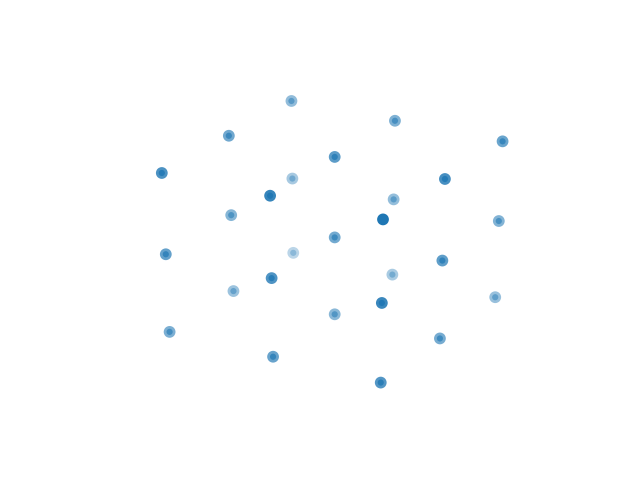
\includegraphics[width=75mm]{cell}
\end{center}
   \captionof{figure}{Reciprocal lattice in k space}\label{cell}\vspace{0.5cm}
   The Brillouin zone will be then as shown in the following figures
   \begin{center}
   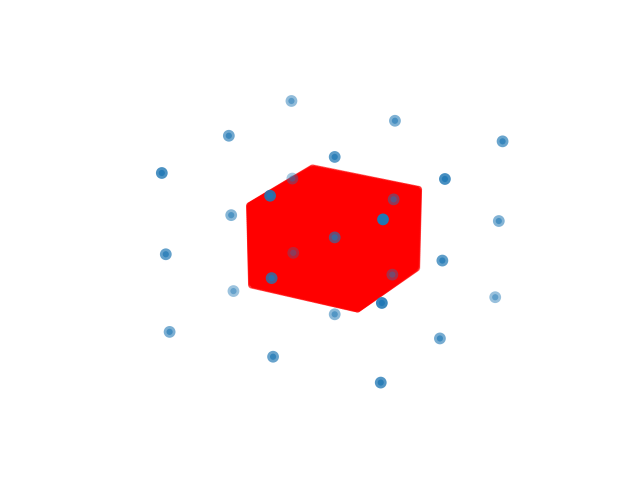
\includegraphics[width=60mm]{brill}
   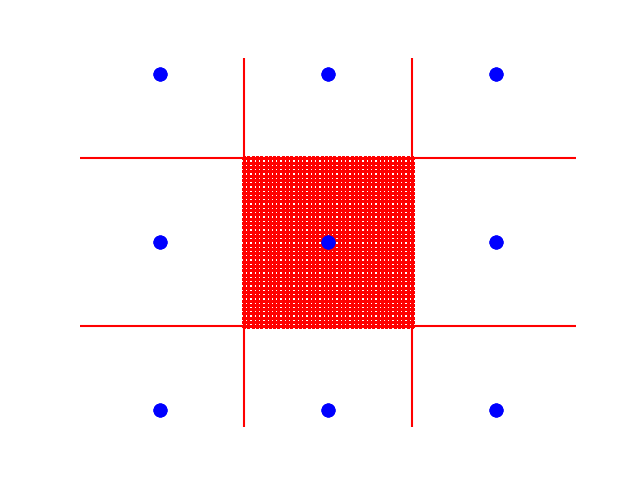
\includegraphics[width=60mm]{contour}
 \end{center}
    \captionof{figure}{Brillouin zone on 3D (left side) and contour plot for $z=0$ (right).}\label{cell}\vspace{0.5cm}

  Finally, how would I find it numerically.

  Honestly I would Google algorithms to find Voronoi-Diagrams because there must be pretty inteligent algorithms to do that. But if that's not a possibility I would to the following
  \begin{enumerate}
    \item Generate a finer mesh.
    \item Travel along the points of this mesh.
    \item For each point detect what lattice points are near.
    \item Measure the distance to all of them.
    \item Assign that mesh point to the closest lattice point.
  \end{enumerate}

\end{solution}
\end{questions}

% \includegraphics[width=75mm]{}
%
%
%  \captionof{figure}{}\label{}\vspace{0.5cm}
